\chapter{人工ニューロンによる演算}

\section{はじめに}

【目的】

本章では人工ニューロン、および多層パーセプトロンを用いた演算について理解します。

【目標】

\begin{itemize}
    \item 人工ニューロンとは何か、およびその原理と構造について説明できること。
    \item 人工ニューロンによる演算について自らの手で計算できること。
    \item 多層パーセプトロン（MLP）とは何か、およびその原理と構造について説明できること。
    \item MLP による演算について、なぜ表現力を増強できるかを説明でき、かつ自らの手で計算できること。
\end{itemize}

【章構成】

\begin{enumerate}
    \item 人工ニューロンとは
    \item 活性化関数
    \item 人工ニューロンによる演算
    \item 例題1：NAND 演算
    \item 多層パーセプトロンとは
    \item 例題2：XOR 演算
\end{enumerate}

\section{神経細胞とは}

% 人工ニューロンの説明

人工ニューロンとは、人工的に神経細胞の動作についてモデル化したものである。
まずは神経細胞の構造と機能について説明する。

神経細胞（ニューロン）は、主に次の構造を持つ。
\begin{itemize}
    \item 細胞体（Soma）。核を持ち、細胞の活動を管理する。細胞膜によって内外が分かれている。
    \item 樹状突起（Dendrite）。他の神経細胞の複数の入力をここで受ける。
    \item 軸索（Axon）。神経細胞の活動を他の神経細胞へ送る。
\end{itemize}

\begin{figure}[tbp]
    \centering
    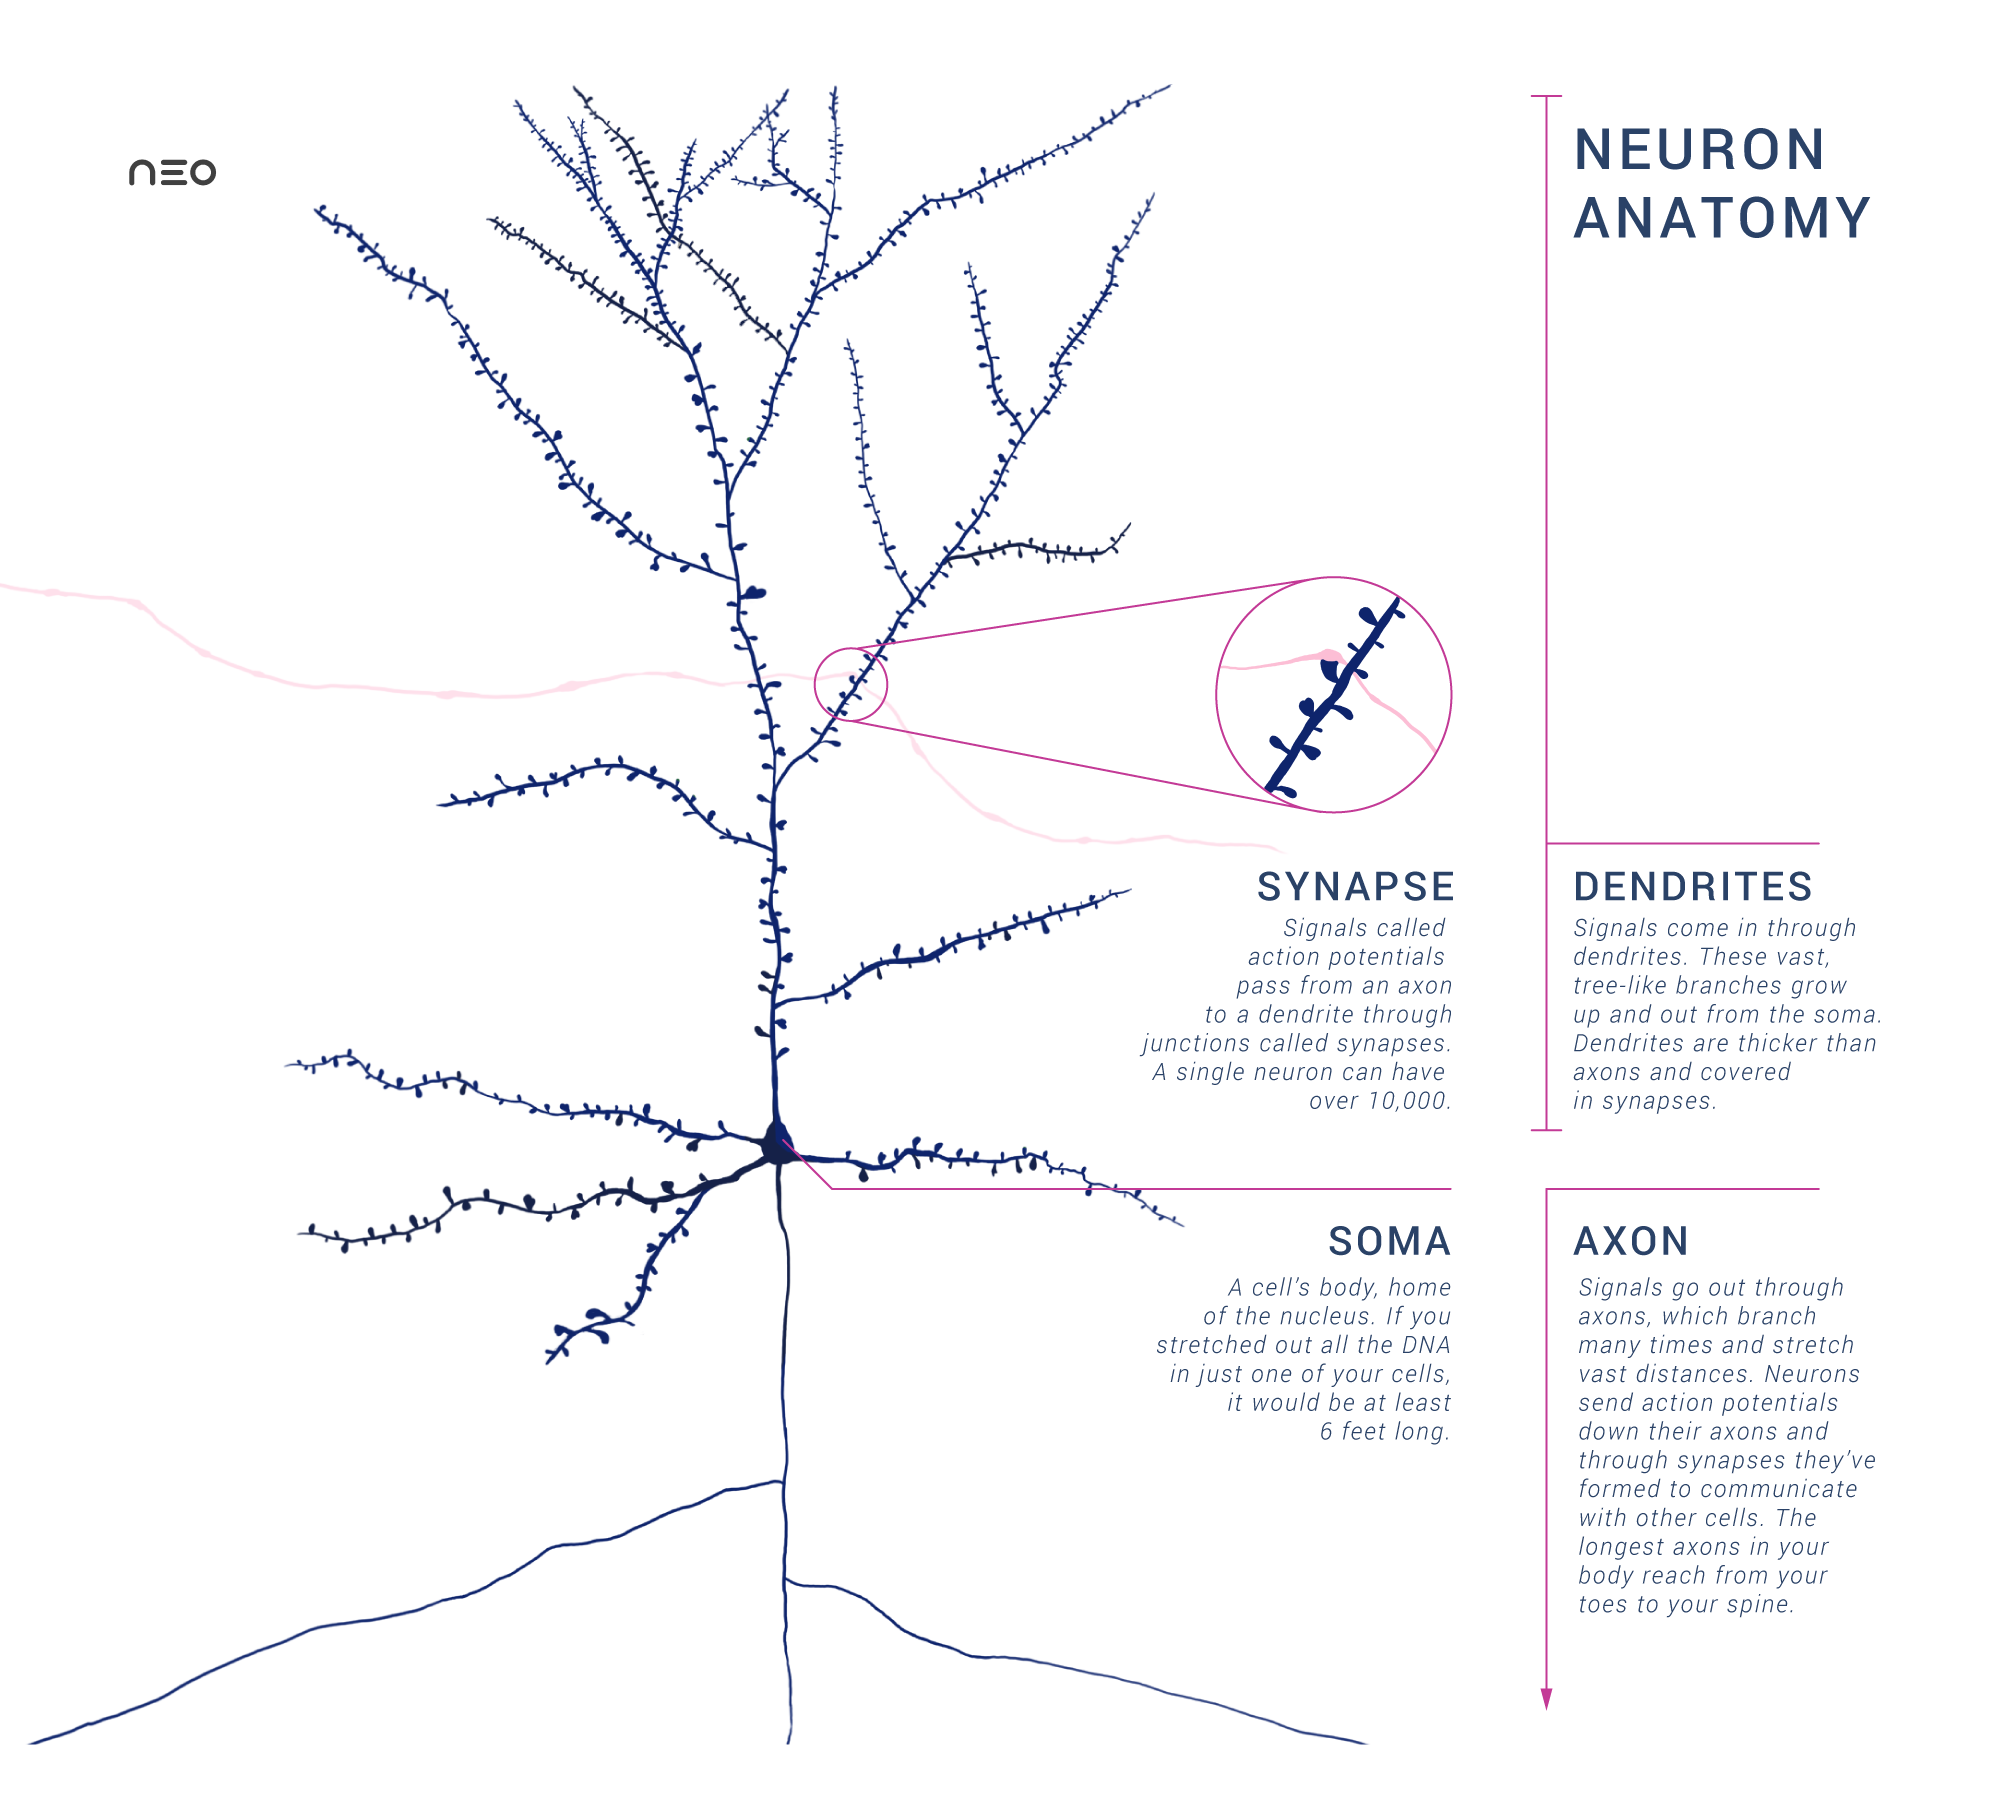
\includegraphics[width=0.8\columnwidth]{src/chap1_neuron/img/Anatomy_of_a_Neuron_with_Synapse.png}
    \caption{単一の衰退神経細胞の概略図。図上部が樹状突起、図下部が軸索を表している。丸で囲われた部分がシナプスを示している。Amyleesterling, CC BY-SA 4.0 via Wikimedia Commons}
 \end{figure}

おおまかに、樹状突起→細胞体→軸索→樹状突起→...として神経細胞の活動を伝える。
この活動の伝搬が神経細胞組織内で行われる情報の伝達を担う。

神経細胞上では、電気的な信号としてその活動を伝搬する。
細胞の外と中では無機イオンの濃度が異なり、細胞膜は内外を電気的に絶縁しており、電気的に安定している。
この電位を静止膜電位といい、約 -70 mV である。
なお、わずかながら内外でイオンのやり取りがあり、この内外のやり取りはチャネルと呼ばれるタンパク質が担っている。
細胞内は K+濃度が、細胞外は Na+濃度が高くなっており、K+の方がNa+に比べて透過性が高い。

% https://www.kango-roo.com/learning/2078/

ここで、神経細胞が他の神経細胞から信号を受け取ったとき、膜電位が正方向へ変化する（脱分極）。
この動作が閾値を超えたとき、カリウムチャネルが閉じ、ナトリウムチャネルが開くことでNa+の透過性が劇的に向上する。
これによりNa+が細胞内に流入し始め、細胞内の電位が上昇する。
細胞内の Na+ 濃度が上昇し、膜電位が約 +40 mV を超えると、ナトリウムチャネルが閉じると同時にカリウムイオンチャネルが開き K+が細胞外へ流出する。
これにより膜電位が低下する（再分極）。
なお、静止膜電位より少し低めまで下がった後（過分極）、静止膜電位まで近づく。
静止膜電位へ近づく間は他の神経細胞からの刺激に反応しづらくなる。
この期間を不応期と呼ぶ。

このような特異的な波形を活動電位といい、活動電位が発生することを発火する、という。
最初の段階である脱分極の閾値について、ここで閾値を超えない場合は神経細胞が発火しない。
一方で、神経細胞へ閾値以上の刺激を与えた場合、活動電位のピークは一定である。
この現象を全か無かの法則という。
神経細胞の活動電位の波形は一定だが、強い刺激には頻繁な発火が起こる、つまり発火頻度で刺激強度を表現している。

このように、神経細胞の軸索を活動電位が伝搬することで軸索末端まで情報を運ぶ。
余談だが、活動電位は軸索の表面を順々に伝わるわけではない。
シュワン細胞という神経細胞とは別の細胞が構成するミエリン鞘が複数個軸索を取り囲んでおり、ミエリン鞘の間には隙間が空いている。
この部分はランヴィエ絞輪と呼ばれ、この部分にナトリウムチャネルが密集している。
この構造を用いて、絶縁体であるミエリン鞘を飛び越えながらランヴィエ絞輪を介して活動電位をより高速に伝達することができる。
これは跳躍伝導と呼ばれ、活動電位を10--100倍ほど高速に伝達することができる。

軸索や樹状突起が結合する部分をシナプス（Synapse）と呼ぶ。
"シナプス" は「留め具」というギリシャ語に由来する。
したがって、軸索--樹状突起間の接触もシナプス（Axodedritic Synapse）、軸索--軸索間の接合もシナプス（Axoaxonic Synapse）、軸索--細胞体間の接合もシナプス（Axosomatic Synapse）と呼ばれる。

シナプスは大きく分けて2つの分類があり、化学物質を受け取る化学シナプスと、電気的な信号を送る電気シナプスがある。
多くのシナプスは化学シナプスであり、アセチルコリンやGABA、ドーパミンといった神経伝達物質を介して情報を伝達する。
化学シナプスは興奮性シナプスと抑制性シナプスに細分される。
名前の通り、興奮性シナプスは前段が発火すると後段の発火を促すものであり、抑制性シナプスは逆に前段が発火すると後段の発火を抑えるものである。

一方で、電気シナプスはギャップ結合と呼ばれる細胞膜間結合をもち、細胞膜間にあるタンパク質によるゲートを介して、無機イオンや水溶性低分子をやり取りし、電気的結合を得られる。

シナプスの結合は神経活動の伝搬頻度によって柔軟に変化する。
これをシナプス可塑性という。
ヘブによって「シナプス前段の発火によりその後段の発火を誘発すると神経細胞同士の結合が強くなる」と提唱された（これをヘブ則という）。
この理論は実際の神経組織において長期増強（LTP; Long-term Potentiation）と呼ばれる現象として確認されている。
これはシナプスの伝達効率が数時間から数か月単位といった長期間増強される。
一方で、この逆として長期抑制（LTD; Long-term Depression）と呼ばれる現象も確認されている。
これは伝達効率の低下が長期にわたって継続されるものである。
これらのような現象が組み合わさって学習や記憶形成に関わっていると考えられている。

% 計算機上で神経細胞の動作を模擬する方法はいくつかある。
% 代表的なものとして、
%   * 電気生理学：Hodgkin-Huxley 方程式（1963 ノーベル医学・生理学賞）
%   * 形式ニューロンに基づく：Perceptron （Rosenblatt による）
%   * CNNの一種：ネオコグニトロン（福島）

% 

\section{人工ニューロンとは}

人工ニューロンは前述した神経細胞のふるまいを計算モデルとして表したものである。
活動電位のような時間方向の変化は模していないことに注意すること。

神経細胞はシナプス結合により情報を集約し、刺激が閾値を超えると発火して後段の神経細胞へ活動電位を伝搬させる。
これを計算モデルとすると、入力信号 ${x_1, ..., x_n}$ から出力信号 $ y $ を生成する素子である。
出力信号 $y$ の算出には各入力信号に対する重み係数 ${w_1, ..., w_n} $ を用いた加重和と、その加重和に対しバイアス項を加算したものを非線形関数 $g(x)$を経て計算される。
この非線形関数は活性化関数と呼ばれ、神経細胞の発火の閾値を模している。

活性化関数を用いることで、人工ニューロンを多段にしたときにより複雑な発火条件の境界を設定できる。
活性化関数が線形関数（ $y=a_1 x_1 + ... a_n x_n $のような多項式モデル ）の場合、人工ニューロンを多段にした場合でも線形関数のみの表現に限定されてしまう。
非線形関数を用いることで、各人工ニューロンの重み係数を調整すれば複雑な境界条件を表現できるようになる。

\section{活性化関数}

活性化関数の例を挙げる。

人工ニューロンの発端であるパーセプトロンでは活性化関数にステップ関数（もしくは階段関数）が用いられた。
ステップ関数とは、数式 \ref{eq:step}で表される。
\begin{equation}
    \label{eq:step}
    g(x) = 
    \begin{cases}
        1 & \text{if $x \ge 0$,} \\
        0 & \text{otherwise}
    \end{cases}
\end{equation}

前述した神経細胞の全か無かの法則を模しているといえる。

また、数式 \ref{eq:sigmoid} で表されるシグモイド関数と呼ばれる関数もよく用いられる。

\begin{equation}
    \label{eq:sigmoid}
    g(x) = \frac{1}{1+e^{-x}}
\end{equation}

これはロジスティック関数の特殊な式であり、ロジスティック関数は上限もしくは下限へ滑らかに向かう関数である。
前述したステップ関数をより滑らかにしたものといえる。

一方で、これらの活性化関数は入力値が大きすぎる、もしくは小さすぎる場合の変化が非常に少ない。
これは次章で扱う勾配消失問題を招くため、最近用いられる活性化関数は ReLU 関数と呼ばれるものが多い。
ReLU 関数は数式 \ref{eq:relu} で表される。

\begin{equation}
    \label{eq:relu}
    g(x) = 
    \begin{cases}
        x & \text{if $x \ge 0$,} \\
        0 & \text{otherwise}
    \end{cases}
\end{equation}

\section{人工ニューロンによる演算}

実際に人工ニューロンによる演算について解説する。

3入力の人工ニューロンについて、
\[ w_0 = 0.5, w_1 = 0.8, w_2 = -0.4, b = 0.2\]

とする。
また、活性化関数にはシグモイド関数を用いるとする。

このとき、入力が

\[ x_0 = 0.1, x_1 = 0.8, x_2 = 0.1\]

だった場合、加重和およびバイアス項の和 $u$ は

\[
    u = 0.5 \times 0.1 + 0.8 \times 0.8 + (-0.4) \times 0.1 + 0.2
    = 0.05 + 0.64 - 0.04 + 0.2
    = 0.85
\]

となり、活性化関数 $g(u)$ の値 $y$は、

\[ y = \frac{1}{1+e^{-u}}
     = \frac{1}{1+e^{-0.85}}
     = 0.70
\]

となる。

\section{例題1：NAND演算}

人工ニューロンは重みを変えることで様々な演算を表現できる。
この例題では 2入力NAND 演算を人工ニューロンで表現する。

入力の重みを $w_0 = -0.5, w_1 = -0.5$ とし、バイアス項 $b$ を 0.8、活性化関数をステップ関数とする。

このとき、2入力の組み合わせとその計算結果を表\ref{tab:nand}に示す。
人工ニューロンによる演算結果とNAND演算の真理値が一致することが分かる。

\begin{table}[htb]
    \begin{center}
        \caption{人工ニューロンによる2入力NAND演算}
        \begin{tabular}{cccc}
            \toprule
            $(x_0, x_1)$ & $u(x)$ & $y$ & 真理値 \\
            \midrule
            (0, 0) &  0.8 & 1 & 1\\
            (0, 1) & 0.3 & 1 &1 \\
            (1, 1) & -0.2 & 0 & 0\\
            (1, 0) & 0.3 & 1 & 1\\ 
            \bottomrule            
        \end{tabular}
        \label{tab:nand}
    \end{center}
\end{table}

\section{多層パーセプトロンとは}

前述した人工ニューロン単体（これを単層パーセプトロンもしくは単純パーセプトロンという）では表現できる演算に限界があることが知られている。
各入力に対し出力に応じてその境界を直線的に分離できるか、という問題に対し、分離可能なものを線形分離可能という。
人工ニューロン単体では線形分離可能な演算しか表現できないため、非線形分離を表現できるよう人工ニューロンを多層的に重ねることで解決が図られてきた。

この人工ニューロンを多層化したものを多層パーセプトロン（MLP; Multi-layer perceptron）という。
MLP は入力層、隠れ層、出力層から構成される。
2層構造であれば、出力層が隠れ層を兼ねる。
前の層の人工ニューロンの出力が次の層の人工ニューロンの入力となり、神経回路網のように信号が伝搬していく。

\section{例題2：XOR演算}

XOR演算は線形分離不可能な演算である。
この例題では 2 層の MLP を用いて XOR 演算を表現する。
この場合、前述した通り入力層（第0層）と出力層（第1層）のみの構成となり、入力層は人工ニューロン2個、出力層は1個で構成される。

入力の重みについて、
\begin{itemize}
    \item 入力層$w_{(0,0)} = (0.8, 0.8), w_{(0,1)} = (-0.8,-0.8)$
    \item 出力層 $w_1 = (0.8, 0.8)$
\end{itemize}

とし、バイアス項 $b$ は、
\begin{itemize}
    \item 入力層 $b_{(0,0)} = -0.5, b_{(0,1)} = 0.9$
    \item 出力層 $b_1 = -1.2$
\end{itemize}
とする。
活性化関数はステップ関数とする。

このとき、2入力の組み合わせとその計算結果を表\ref{tab:xor}に示す。
人工ニューロンによる演算結果とXOR演算の真理値が一致することが分かる。

\begin{table}[htb]
    \begin{center}
        \caption{2層MLPによる2入力XOR演算}
        \begin{tabular}{cccccc}
            \toprule
            $(x_0, x_1)$ & $(u_{(0,0)}, u_{(0,1)})$ & $(y_{(0,0)}, y_{(0,1)})$ & $u_1$ & $y_1$ & 真理値 \\
            \midrule
            (0, 0) & (-0.5, 0.9) & (0, 1) & -0.4 & 0 &0\\
            (0, 1) & (0.3, 0.1) & (1, 1) & 0.4 & 1 & 1 \\
            (1, 1) & (1.1, -0.7) & (1,0) & -0.4 & 0 & 0\\
            (1, 0) & (0.3, 0.1) & (1, 1) & 0.4 & 1 & 1\\ 
            \bottomrule            
        \end{tabular}
        \label{tab:xor}
    \end{center}
\end{table}

なお、各人工ニューロンは入力層 (0,0) が OR演算、(0,1) が NAND演算、出力層がAND演算を模している。 
この構成は実際の論理素子による XOR 演算の構成と同等である。

\section{演習：MLPの設計}

Python で MLP を設計する。

MLP は次のクラス構成とする。

\begin{itemize}
    \item \textbf{Neuron}クラス。人工ニューロンの演算を行う。
    \item \textbf{Layer}クラス。\textbf{Neuron}オブジェクトを組み合わせ1層分の構成を表現する。
    \item \textbf{NeuralNetwork}クラス。\textbf{Layer}クラスを組み合わせ MLP を表現する。
\end{itemize}

これらのクラスに加え、実行時に必要な引数処理などを行うための\textbf{Main}クラスを設ける。

詳細は別紙に示す。